% ==============================================================================
% PG - Nome do Aluno
% Capítulo 4 - Avaliação
% ==============================================================================
\chapter{Apresentação e Avaliação da Proposta}
\label{sec-avaliacao}

% Este capítulo deve ser incluso na monografia quando tiver sido realizado algum tipo de avaliação da proposta que requeira uma descrição detalhada (por exemplo, experimentos, simulações, etc.) O capítulo deve apresentar a avaliação realizada, deixando claro qual foi objetivo da avaliação, os passos realizados, os resultados obtidos e a interpretação desses resultados considerando o objetivo inicial. Em casos em que a avaliação realizada não demande um capítulo dedicado a ela (por ser muito simples ou pequena, por exemplo), ela pode ser tratada em uma seção específica no capítulo anterior.


Este capítulo está dividido em duas partes principais. Na primeira, são apresentadas as telas principais do jogo, desenvolvidas como resultado final do processo de criação. Durante a exibição das telas serão feitos comentários breves sobre o que está sendo mostrado. Na segunda parte serão analisados os resultados da pesquisa que foi realizado através de um formulário. 

\section{Apresentação da Aplicação}
A figura \ref{fig:home-super-labes-world} apresenta a tela inicial ao executar o programa. Nessa tela é possível iniciar um novo jogo, abrir a tela de créditos que contém o link para o repositório do Github com mais informações, abrir a tela de controles do \textit{game}, ou sair do jogo.
\begin{figure}[h!]
    \centering
    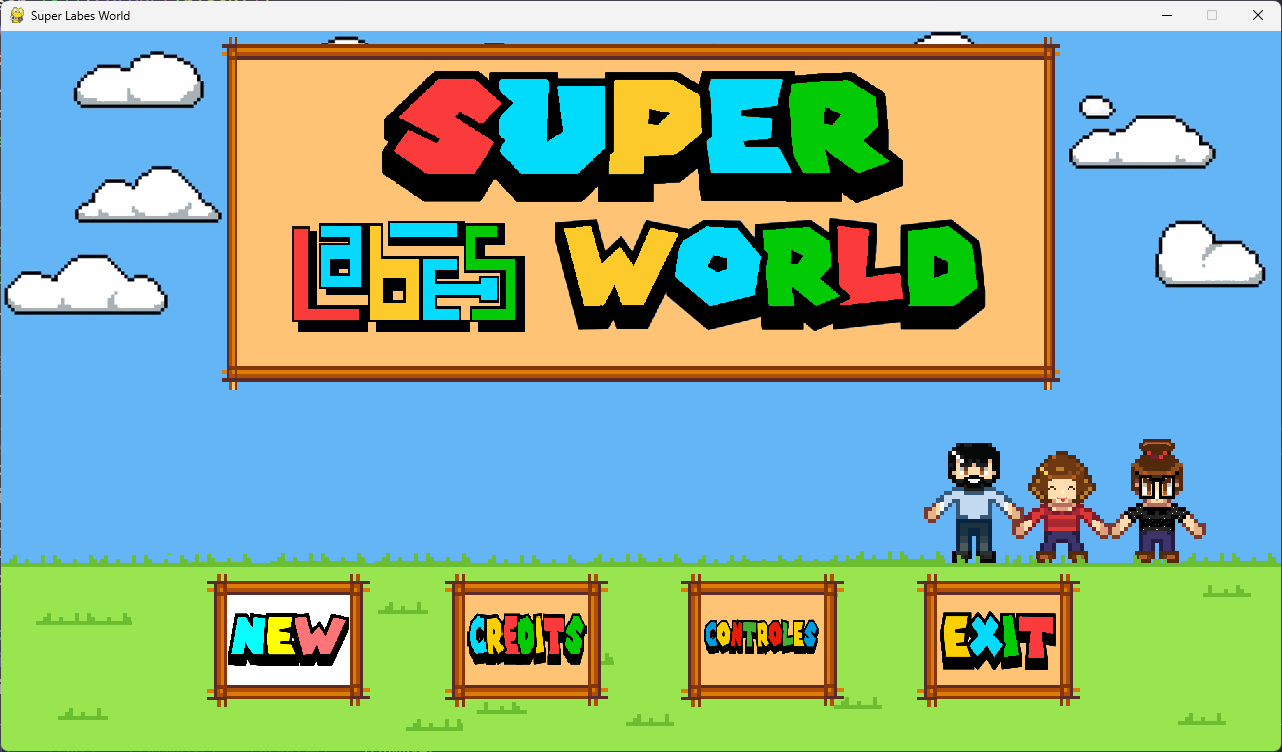
\includegraphics[width=1\linewidth]{figuras/home-super-labes-world.png}
    \caption{Figura ilustrando a home do jogo}
    \label{fig:home-super-labes-world}
\end{figure}

 \newpage
 A próxima tela ilustrada na figura \ref{fig:inventory} mostra como é o \textit{layout} de inventário do jogo. nela é possível ver os items que o jogador carrega e a descrição, o limite do inventário são 30 items. 
\begin{figure}[h!]
    \centering
    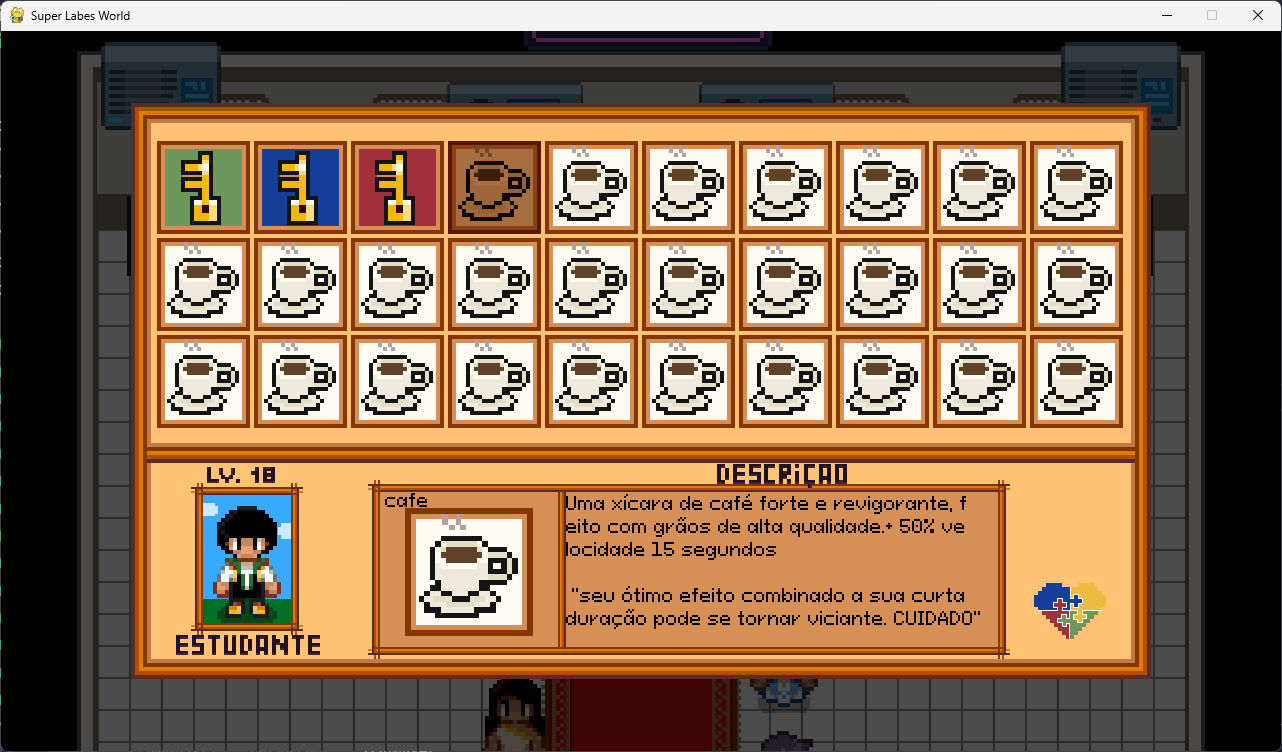
\includegraphics[width=1\linewidth]{figuras/inventory.png}
    \caption{Figura ilustrando o inventário do jogo}
    \label{fig:inventory}
\end{figure}

\clearpage
A figura a seguir \ref{fig:dialog} mostra o jogador interagindo com um dos chefes do jogo antes de entrar em uma batalha.

\begin{figure}[h!]
    \centering
    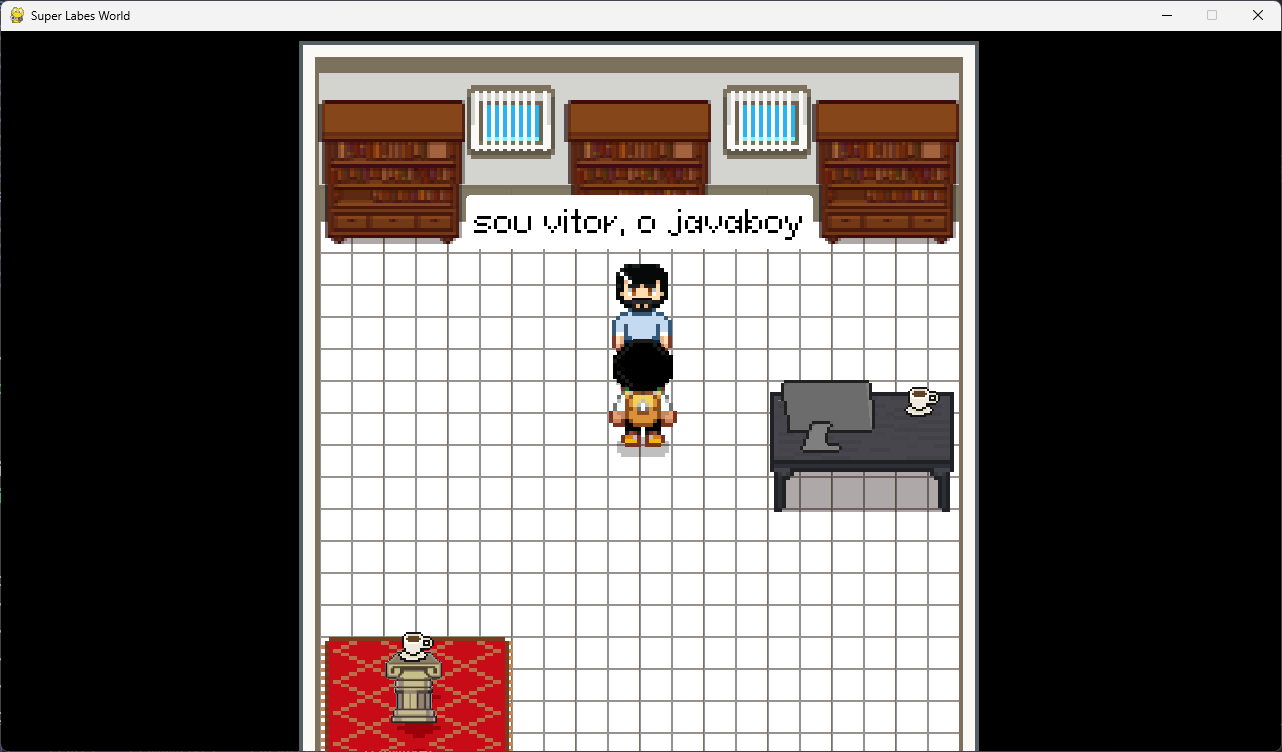
\includegraphics[width=1\linewidth]{figuras/dialog.png}
    \caption{Ilustração de um diálogo do Super Labes World}
    \label{fig:dialog}
\end{figure}
\newpage
Na figura \ref{fig:battle} podemos ver como é a interface da mecânica principal de jogo a batalha de questões. O retângulo superior esquerdo (1) ilustra a pergunta que o jogador tem que responder, o retângulo superior direito (2) mostra o texto dito pelo chefe ao responder a questão, o retângulo intermediário (3) mostra as informações do chefe, os retângulos inferiores vermelho, amarelo, verde e azul (4) são as alternativas a serem escolhidas pelo jogador. Cada opção selecionada altera o texto escrito no retângulo inferior esquerdo de cor branca (5), que é a descrição da resposta. 

\begin{figure}[h!]
    \centering
    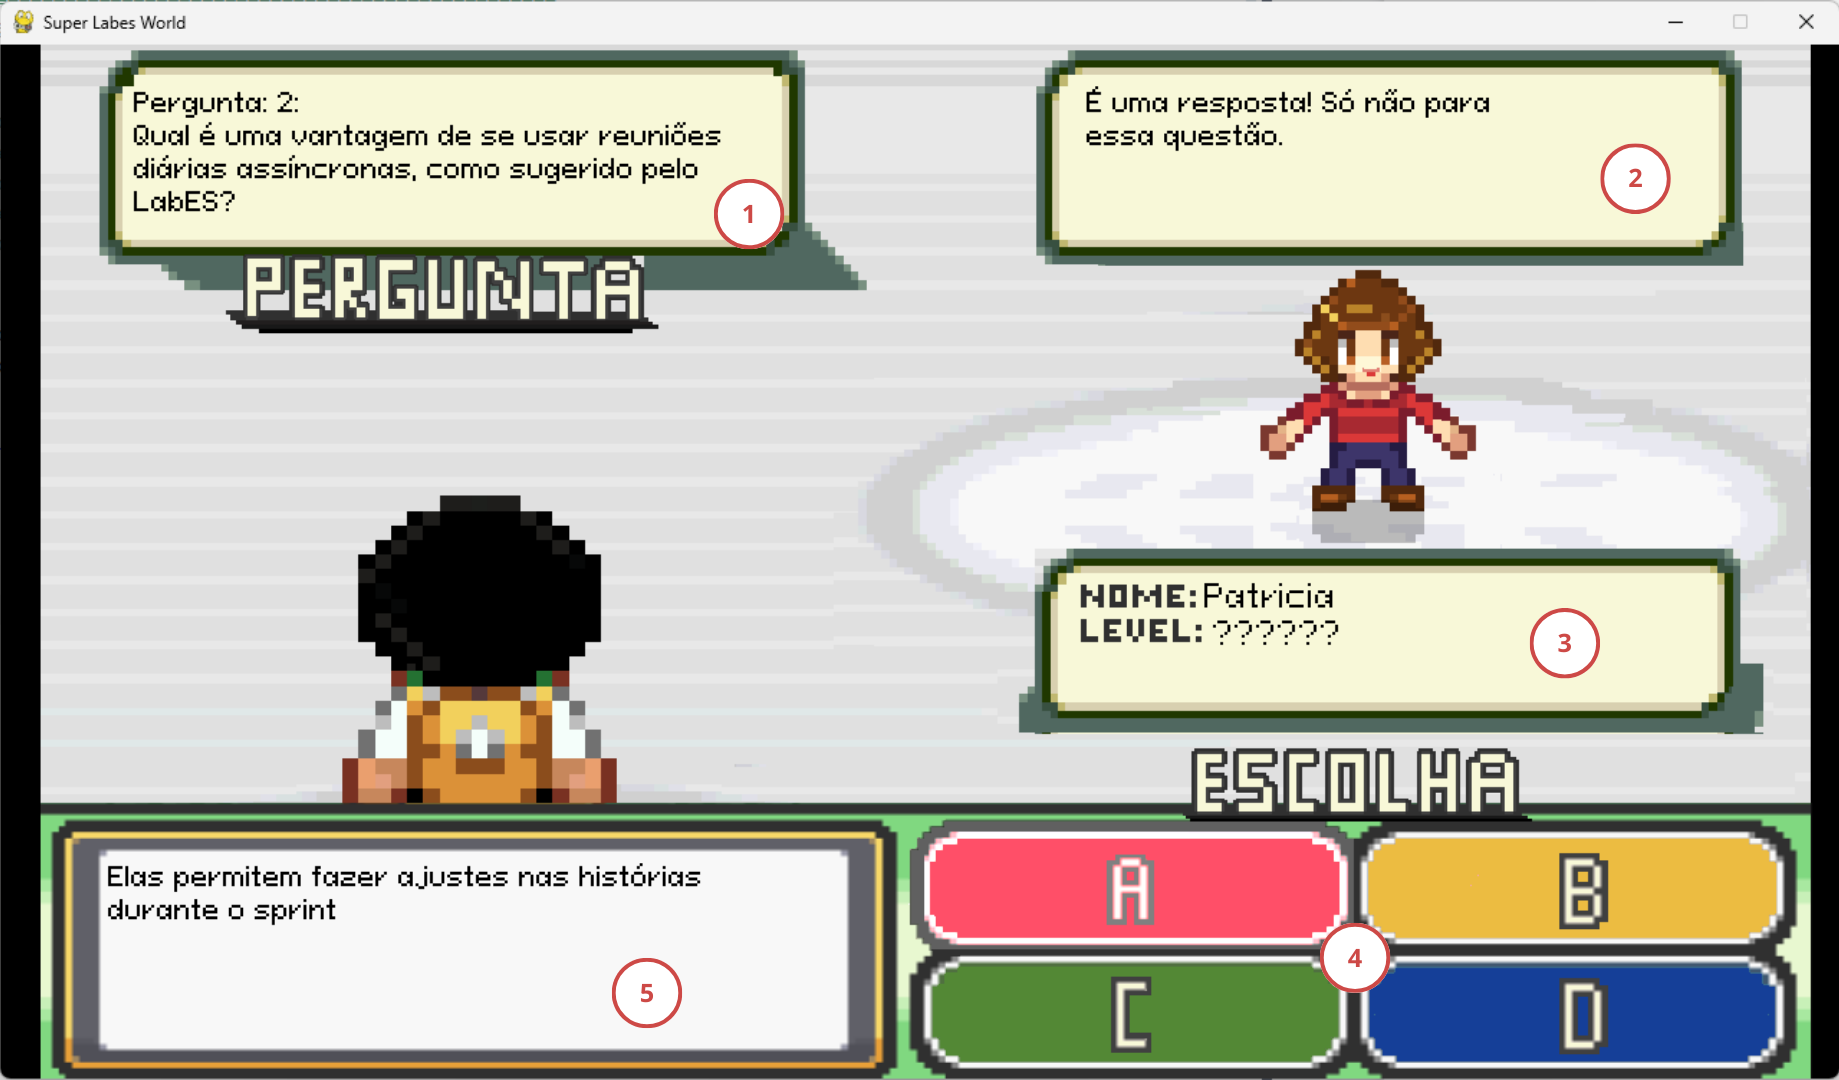
\includegraphics[width=1\linewidth]{figuras/battle.png}
    \caption{Ilustração do sistema de batalha do \textit{game}}
    \label{fig:battle}
\end{figure}
\newpage
Na figura \ref{fig:computer} pode ser vista a interface de computador do jogo, nela é possível o jogador estudar através do jogo. Esse menu contém vários \textit{links} para materiais de estudo que são uteis para vencer o jogo. Caso o jogador abra essa interface após uma batalha com um professor, o computador terá somente os \textit{links} associados as perguntas que o usuário errou.
\begin{figure}
    \centering
    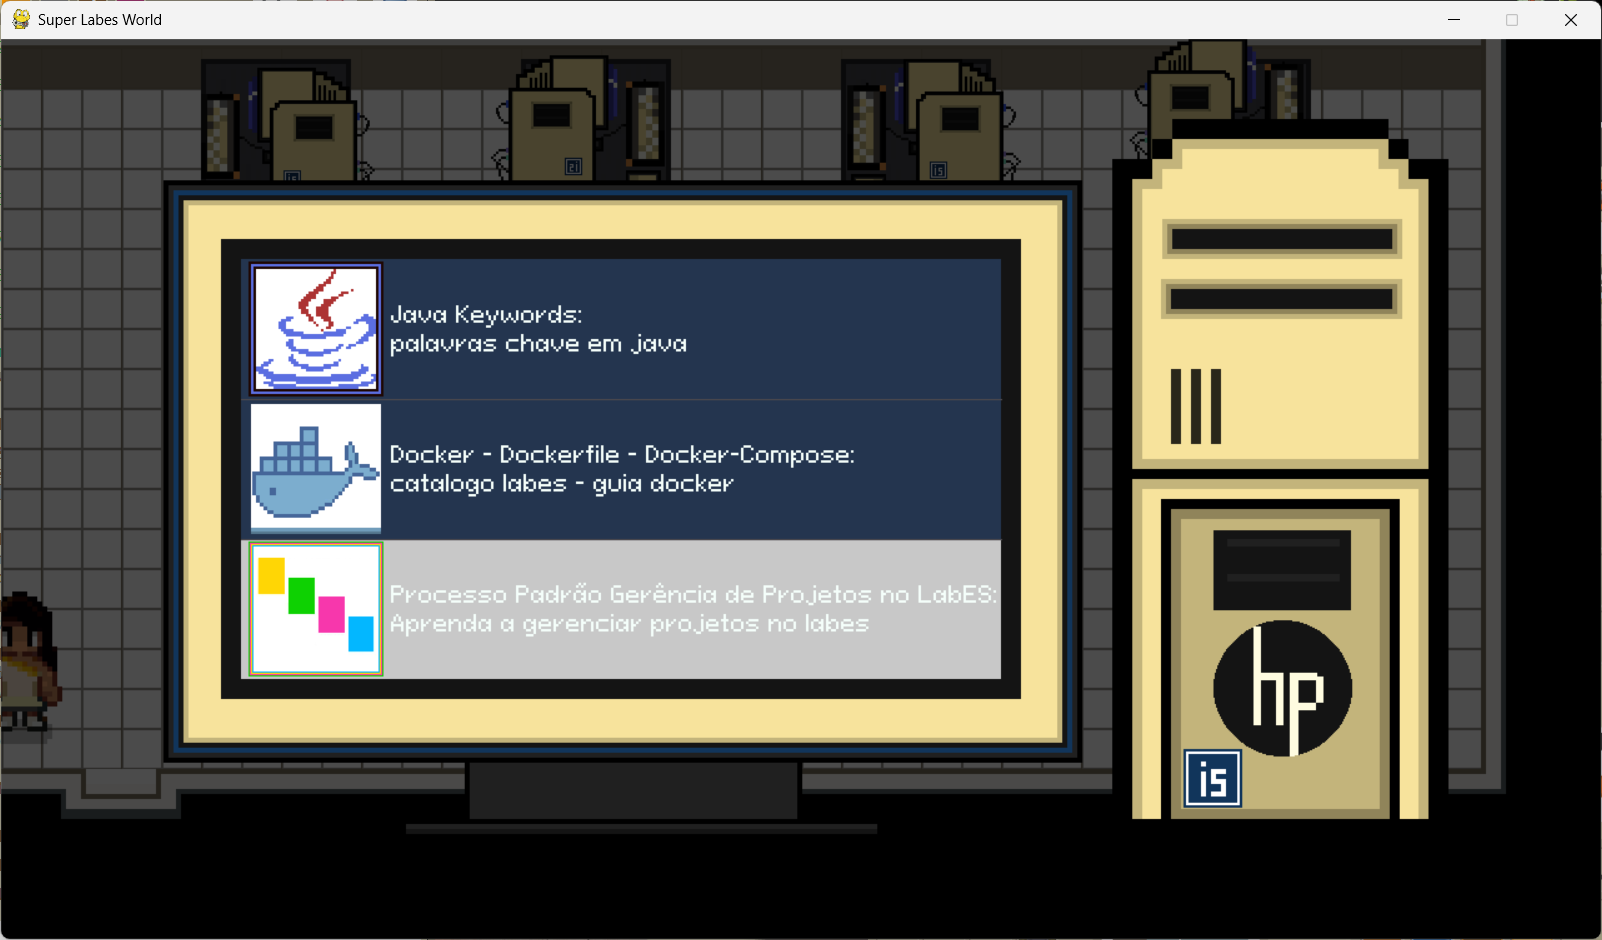
\includegraphics[width=1\linewidth]{figuras/computer.png}
    \caption{\textit{Layout} do computador no jogo usado para acessar \textit{links} de materiais de estudo}
    \label{fig:computer}
\end{figure}

\section{Avaliação do Jogo}
\label{sec:avaliacao-do-jogo}
Com o término do desenvolvimento do jogo, deu-se início à etapa de avaliação e validação do jogo com os principais potenciais usuários desse sistema, os membros do LabES. O objetivo dessa fase foi analisar a jogabilidade em um contexto de uso real, e também obter métricas, com relação aos parâmetros básicos de qualidade de software e dos objetivos propostos pelo jogo. Após os usuários terminarem de jogar, foi-lhes disponibilizado um formulário e tivemos os seguintes resultados.

\begin{figure}[h!]
    \centering
    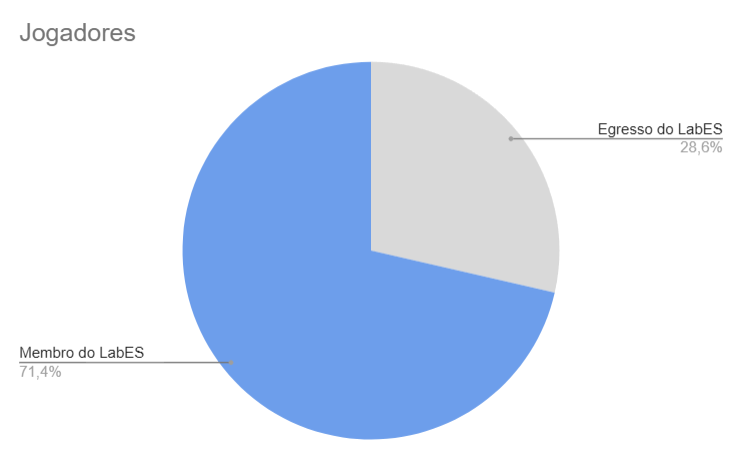
\includegraphics[width=0.8\linewidth]{figuras/players-pizza.png}
    \caption{Percentual de jogadores membros e egressos do LabES que participaram da pesquisa}
    \label{fig:players-pizza}
\end{figure}

A Figura \ref{fig:players-pizza} mostra o percentual dos usuários que jogaram o Super Labes World, a maioria são membros atualmente no LabES. Dentre os que concluíram o jogo, o tempo médio para finaliza-lo foi 35 minutos. O jogo em sua versão atual conta três chefes sendo dois com 10 perguntas, e um com 11, totalizando 31 perguntas de múltipla escolha com quatro alternativas. 

\begin{figure}[h!]
    \centering
    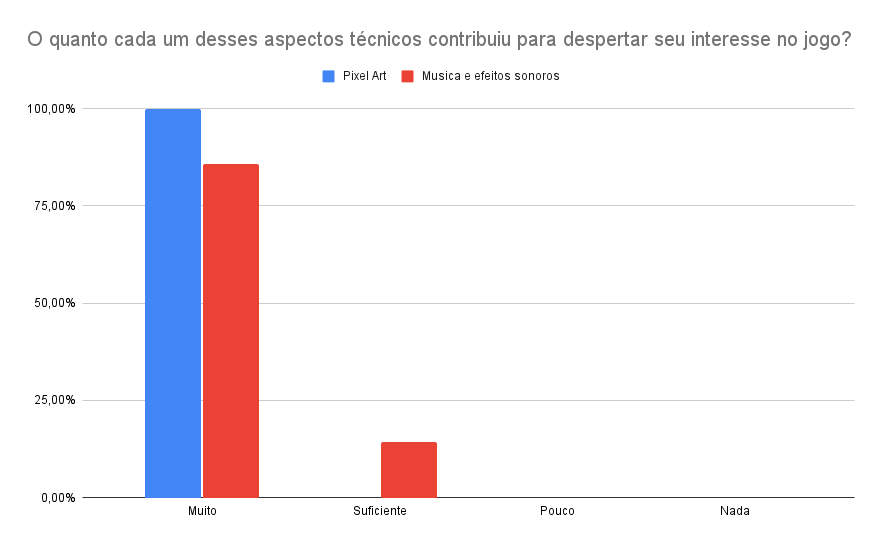
\includegraphics[width=1\linewidth]{figuras/graph-2.png}
    \caption{Gráfico de barras ilustrando os resultados da pesquisa de sobre interesses técnicos no jogo}
    \label{fig:graph-2}
\end{figure}
\clearpage
O uso da \textit{Pixel Art} foi um grande motivador de interesse aos usuários, 100\% dos jogadores responderam que esse aspecto foi relevante para o seu engajamento no jogo. Quanto a trilha sonora foi importante para 85\% desses mesmos usuários.

\begin{figure}[h!]
    \centering
    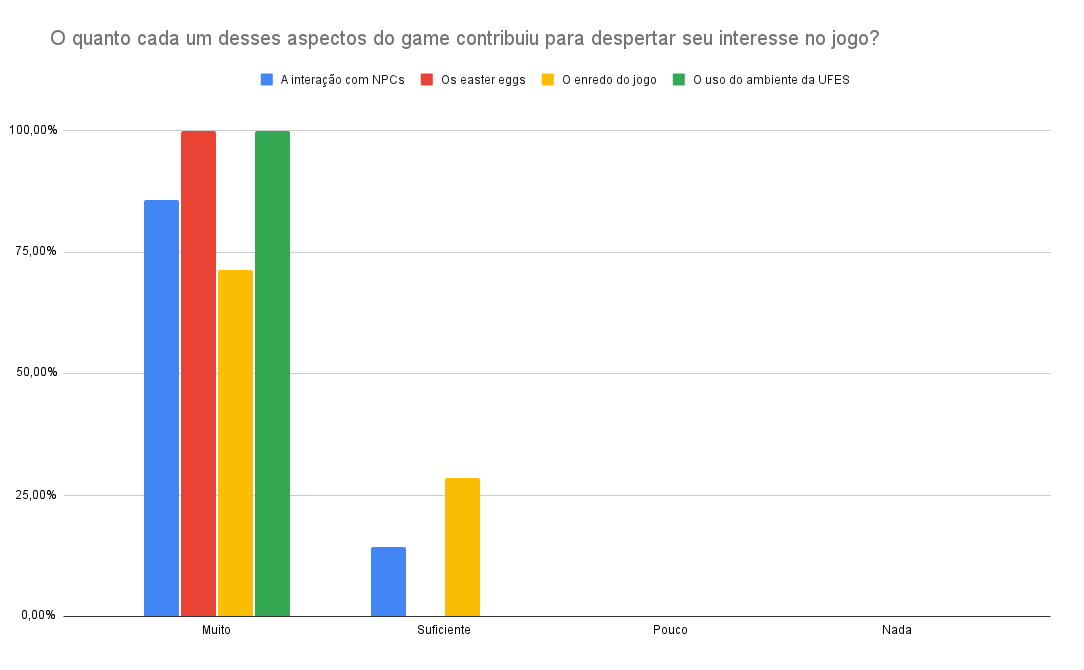
\includegraphics[width=1\linewidth]{figuras/graph-3.png}
    \caption{Gráfico de barras ilustrando os resultados da pesquisa de sobre aspectos do jogo}
    \label{fig:graph-3}
\end{figure}

Os \textit{easter eggs} (segredos de caráter humorísticos), e a ambientação do jogo se passar na UFES também foram unânimes em aceitação entre os jogadores. A figura \ref{fig:graph-3} mostra o resultado da pesquisa em relação a aspectos do \textit{game} que despertaram o interesse. 

\clearpage
A avaliação geral de todos os jogadores sobre o jogo ficou com uma média 4.71 de 5, no geral a maioria teve uma experiencia positiva e agradável com ao jogar o Super Labes World. Todos os entrevistados responderam sim para a pergunta: ''você acredita que video-game é uma boa forma de aprendizado?'' e  '' O Super Labes World o estimulou a aprender?''. Essas foram perguntas chave para motivação desse trabalho. 

A tabela \ref{tbl-relatos-jogo} mostra alguns depoimentos de jogadores que concluíram o jogo.
\begin{table}[h!]
	\caption{Tabela com alguns relatos sobre a seguinte pergunta '' Você acredita que o jogo foi uma boa forma de aprendizado? ''.}
	\label{tbl-relatos-jogo}
	\centering
	\renewcommand{\arraystretch}{2}
	\begin{small}
		\begin{tabular}{ | p{35mm} | p{100mm} |}\hline
			  % \centering{\textbf{Classe}} & \textbf{Descrição}  \\\hline
			\centering{Pessoa 1} & ''Às vezes, quando estamos muito atarefados com as coisas da faculdade, a vontade de aprender não é suficiente. A proposta de um jogo pode ser boa para um aprendizado mais tranquilo e atrativo e que não dê a sensação de "peso" que estudo pra provas às vezes podem dar.'' \\\hline
			\centering{Pessoa 2} & ''É uma boa forma de aprender coisas simples, que muitas vezes as pessoas que já estão no projeto E podem acabar esquecendo se ensinar.'' \\\hline
			\centering{Pessoa 3} & ''Realmente me forçou a pesquisar sobre e ler as recomendações para avançar no jogo.'' \\\hline
                \centering{Pessoa 4} & ''O jogo cria objetivos mais palpáveis e de curto prazo com recompensas instantâneas facilitando o senso de progressão e estimulando o estudo sobre o tema do jogo.'' \\\hline
		\end{tabular}
	\end{small}
\end{table}

Por fim a pergunta fundamental e que foi a principal motivadora para o desenvolvimento desse trabalho foi sobre foi respondida na figura 

\begin{figure}[h!]
    \centering
    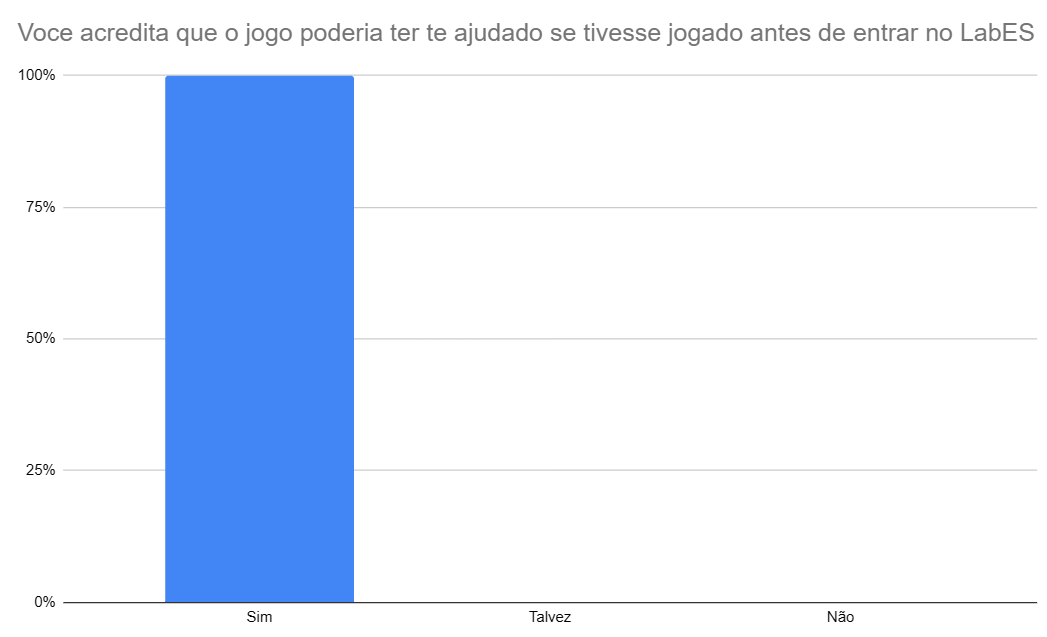
\includegraphics[width=0.81\linewidth]{figuras/graph-1.png}
    \caption{Gráfico de barras ilustrando o resultado para a pergunta motivadora para desenvolvimento do jogo}
    \label{fig:graph-1}
\end{figure}